\PassOptionsToClass{
  title={GLM Hessian Notes},
  header,
  letterpaper,
  12pt
}{hw-scrartcl}

\documentclass{hw-scrartcl}

\usepackage{prob-style}
\usepackage{my-theorems}

\begin{document}
\maketitle
\section{Definitions and set-up}
We will consider a glm to be a collection of samples \(\{(x_i, y_i)\}_{i=1}^n \subseteq \R^p \times \R\), where
\[
  y_i|x_i
  \sim P_{x_i \transp \beta}
\]
for \(\{P_\eta | \eta \in H\}\) a \(1\)-parameter exponential family indexed by a natural parameter \(\eta\) with densities
\[
  p_\eta(y)
  = \exp\{\eta y - \psi(\eta)\} p_0(y).
\]

Conditional on \(X\), the matrix whose rows are the \(x_i\)s, \(y\) thus has density
\[
  f_\beta(y)
  = \exp\Big\{\beta\transp (X\transp y) - \sum_{i=1}^n \psi(x_i\transp \beta)\Big\} f_0(y).
\]

The likelihood and corresponding derivatives are then given by
\begin{align*}
  \ell(\beta)
  &= \beta\transp (X\transp y) - \sum_{i=1}^n \psi(x_i\transp \beta) + \log f_0(y), \\
  \nabla \ell(\beta)
  &= X\transp y - \sum_{i=1}^n \psi'(x_i\transp \beta) x_i, \\
  \nabla^2 \ell(\beta)
  &= -\sum_{i=1}^n x_i \psi''(x_i\transp \beta) x_t \transp \\
  &= -X\transp D_{X\beta} X,
\end{align*}
where \(D_{X\beta}\) is the diagonal matrix with \(i\)th entry \(\psi''(x_i\transp \beta)\), which is the conditional variance of \(y_i\).

Notice in particular that the Hessian of the log-likelihood has no dependence on \(y\) --- a feature unique to GLMs.

\section{The Hessian at the MLE}
We are interested in the spectrum of \(\nabla^2 \ell(\hat{\beta})\). Notice from the previous remark that this depends on \(y\) only through \(\hat{\beta}\). In particular, if \(\hat{\beta}\) is close to the true \(\beta_0\), we can expect that \(\nabla^2 \ell(\hat{\beta})\) is close to \(\nabla^2 \ell(\beta_0)\), and so doesn't depend on \(y\). In this case, the Hessian would be unaffected by using \(y\) to learn \(\beta\).

To show this convergence, we will study the distance between eigenvalue distributions of matrices of the form \(X\transp D X\). In particular, for any Lipschitz function \(f\), we have that
\begin{align*}
  \abs[\Big]{\int f(\lambda) \diff \mu_u(\lambda) - \int f(\lambda) \diff \mu_v(\lambda)}
  &\leq \frac{1}{n} \sum_{i=1}^n \abs{f(\lambda_i) - f(\nu_i)} \\
  &\leq \frac{1}{n} \sum_{i=1}^n \abs{\lambda_i - \nu_i} \\
  &\leq \frac{1}{n} \norm{X\transp (D_u - D_v) X}_1 \\
  &\leq \frac{1}{n} \norm{D_u - D_v}_1 \norm{X}_\infty^2 \\
  &= \norm{u - v}_1 \frac{1}{n} \norm{X}_\infty^2.
\end{align*}

If \(X\) is an \(n \times p\) matrix of iid normals, \(n\rightarrow \infty\) with \(p\) fixed, we have that \(\norm{X}_\infty^2 \sim n\) and \(\norm{\hat{\beta} - \beta_0} \rightarrow 0\). In this case, we have that
\[
  \mu_{\hat{\beta}} \rightarrow \mu_{\beta_0}
\]
almost surely in Wasserstein distance (and hence, for example, weakly).

\section{Logistic regression}
Consider the logistic setting where \(y_i\) takes values \(\{\pm 1\}\). In this case, we have that
\[
  \psi''(\eta)
  = \frac{1}{\cosh^2 \eta},
\]
and therefore
\[
  \nabla^2 \ell(\beta)
  = -\sum_{i=1}^n \frac{x_i x_i\transp}{\cosh^2 x_i\transp \beta}.
\]

For simplicity, consider the case where \(x_{ij}\) are iid normals and \(\beta \in \Unif(S^{p-1})\) is constant. Let \(P = I - \beta\beta\transp\) be the projection onto the subspace orthogonal to \(\beta\). We can then write
\[
  \nabla^2 \ell(\beta)
  = -\sum_{i=1}^n \frac{(P x_i) x_i\transp}{\cosh^2 x_i\transp \beta} - \beta \sum_{i=1}^n \frac{(\beta\transp x_i) x_i\transp}{\cosh^2 x_i\transp \beta}.
\]

Asymptotically, the second

\section{Broad strokes argument for semicircle law for small covariance matrices}
First, notice that for a matrix \(A\) and scalar \(\lambda\), we have that
\begin{align*}
  s_{\lambda A}(z)
  &= \frac{1}{d} \Tr(\lambda A - z\Id)^{-1} \\
  &= \lambda^{-1}\frac{1}{d} \Tr(A - (z/\lambda) \Id)^{-1}\\
  &= \lambda^{-1} s_A(z \lambda^{-1}).
\end{align*}

From this it follows that
\[
  z_{\lambda A}(s) = \lambda z_A(\lambda s),
  \qquad
  R_{\lambda A}(s) = \lambda R_A(\lambda).
\]

Now, we have that, asymptotically, \(\norm{x_i}^2 \sim p\). Hence, we write that
\begin{align*}
  s_{x_i x_i\transp/p}(z)
  &= \frac{1}{p}\Tr\Big(\frac{1}{p}x_i x_i\transp - z\Id\Big)^{-1} \\
  &= \frac{1}{p}\Big[\frac{1}{\norm{x_i}^2/p - z} - \frac{p-1}{z}\Big] \\
  &\approx \frac{1}{p}\Big[\frac{1}{1 - z} - \frac{p-1}{z}\Big].
\end{align*}

For large \(p\), it follow that then
\begin{align*}
  z_{x_i x_i\transp/p}(s)
  &\approx -\frac{1}{s} + \frac{1}{p(1 + s)}, \\
  R_{x_i x_i\transp/p}(s)
  &\approx \frac{1}{p(1 - s)}.
\end{align*}

Assuming the corresponding convolution is indeed asymptotically free, we have that
\begin{align*}
  R_{\sum_{i=1}^n x_i x_i\transp/p}(s)
  &\approx \frac{n}{p(1-s)}, \\
  R_{\frac{1}{2\sqrt{np}}\sum_{i=1}^n x_i x_i\transp}(s)
  &= \frac{1}{2}\sqrt{\frac{p}{n}} R_{\sum_{i=1}^n x_i x_i\transp/p}\Big(\frac{1}{2}\sqrt{\frac{p}{n}}s\Big) \\
  &\approx  \sqrt{\frac{n}{p}}\frac{1}{2 - s\sqrt{n/p}}.
\end{align*}

Finally, since \(R_I(z) = 1\), we have that
\begin{align*}
  R_{\frac{1}{2\sqrt{np}}(\sum_{i=1}^n x_i x_i\transp - nI)}(s)
  &\approx \sqrt{\frac{n}{p}}\frac{1}{2 - s\sqrt{p/n}} - \frac{1}{2}\sqrt{\frac{n}{p}} \\
  &= \sqrt{\frac{n}{p}} \frac{s\sqrt{p/n}}{2(2 - s\sqrt{p/n})}\\
  &= \frac{s}{2(2 - s\sqrt{p/n})} \\
  &\approx \frac{s}{4}.
\end{align*}

Indeed, this is the \(R\)-transform of the semicircle law on \([-1, 1]\). Notice that is seems that the \(x_i\) having internal dependence causes no problems, except possibly rendering the sum asymptotically free, as long as \(\norm{x_i}^2 \sim p\).

To generalise, suppose that instead, \(\norm{x_i}^2 \sim p W_i\) with \(W_i > 0\) and \(\E W_i = \mu\). We then have that
\[
  R_{x_i x_i\transp/p}(s)
  \approx \frac{w_i}{p(1 - s w_i)},
\]
which renders, for large \(n\),
\begin{align*}
  R_{\sum_{i=1}^n x_i x_i\transp/p}(s)
  &= \sum_{i=1}^n \frac{w_i}{p(1 - s w_i)} \\
  &\approx \frac{n}{p} \E\Big[\frac{W}{1 - sW}\Big], \\
  R_{\frac{1}{2\sqrt{np}}\sum_{i=1}^n x_i x_i\transp}(s)
  &\approx \sqrt{\frac{n}{p}}\E\Big[\frac{W}{2 - sW\sqrt{p/n}}\Big], \\
  R_{\frac{1}{2\sqrt{np}}(\sum_{i=1}^n x_i x_i\transp - n\mu I)}(s)
  &\approx \sqrt{\frac{n}{p}}\bigg(\E\Big[\frac{W}{2 - sW\sqrt{n/p}}\Big] - \frac{\mu}{2}\bigg) \\
  &= \sqrt{\frac{n}{p}} \E\Big[\frac{s W^2 \sqrt{p/n}}{2(2 - sW\sqrt{n/p})}\Big] \\
  &\approx \frac{s}{4} \E W^2 \\
  &= \frac{(s\sqrt{\E W^2})}{4} \sqrt{\E W^2}.
\end{align*}

Thus, we have that the ESD of
\[
  \frac{1}{\sqrt{\E W^2}} \frac{1}{2\sqrt{np}}\Big(\sum_{i=1}^n x_i x_i\transp - n\mu\Id\Big)
\]
converges to the semicircle law.

\begin{figure}
  \centering
  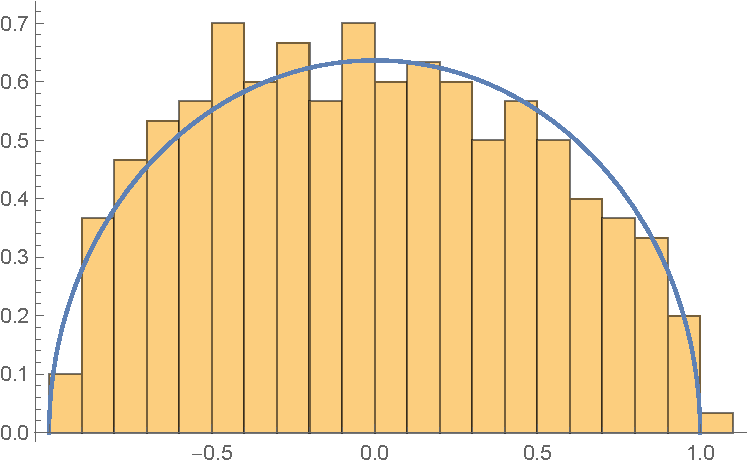
\includegraphics[width=\linewidth]{figures/corr-covmat-eigenvalues}
  \caption{Eigenvalues of a scaled and centred sample covariance matrix.}
  \label{fig:covmat-eig}
\end{figure}

We see this result supported empirically in \cref{fig:covmat-eig} which shows the abovse scaling applied to the matrix \(X D X\transp\), where \(X\) are \(p\times n\) iid standard Gaussians, \(D\) is a diagonal matrix with diagonal entries \(1/\cosh^2 W_i\), for standard normal \(W_i\) and \(n = 30000, p = 300\).

Applying this result to the case of logistic regression, we expect to see a single eigenvalue at \(-n\E(W^2/\cosh^2 W)\) and the bulk conforming to a semicircle law supported on \(n\mu \pm 2\sigma \sqrt{np}\). With the same parameters as in the previous simulation, we see in \cref{fig:logistic-semicircle} that this is largely accurate.
\begin{figure}
  \centering
  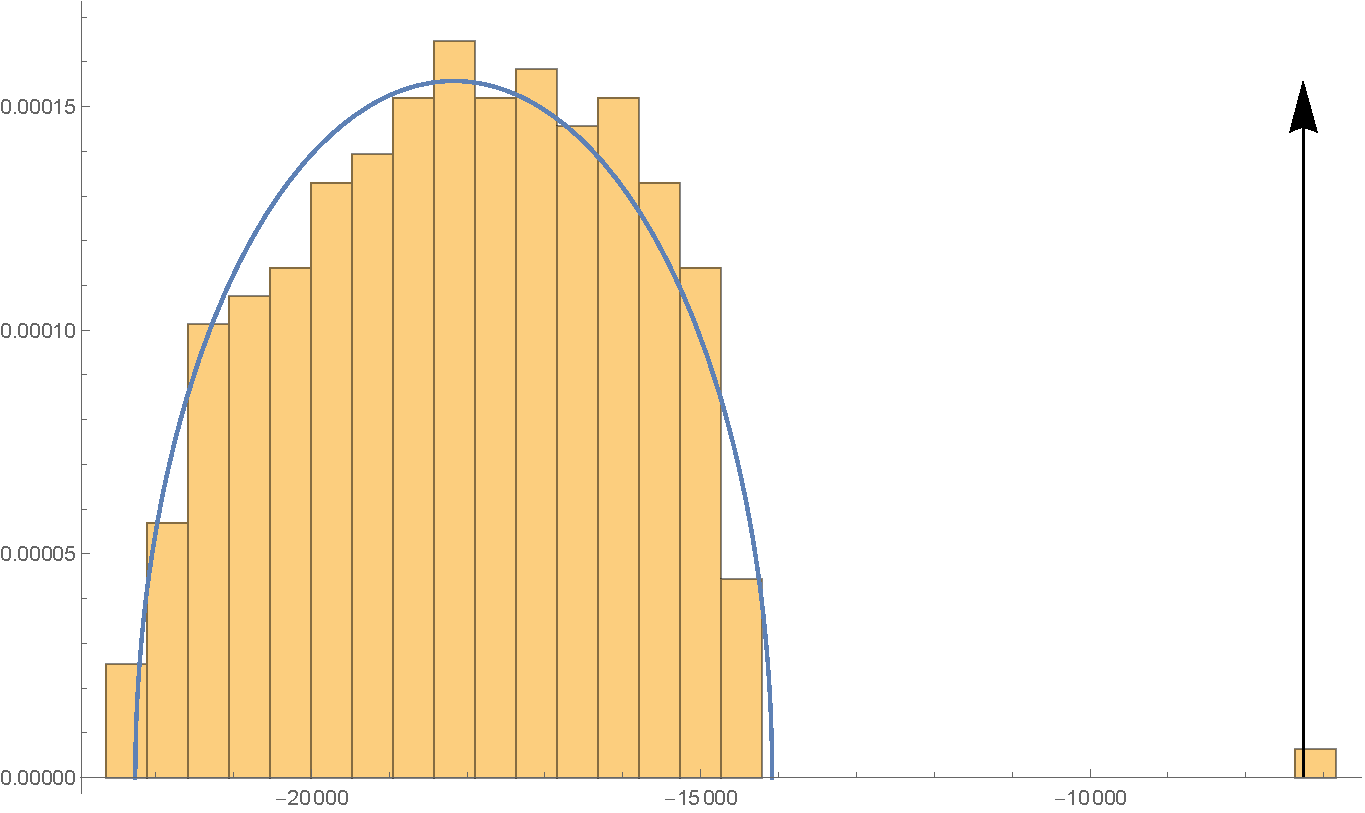
\includegraphics[width=\linewidth]{figures/logistic-eigenvalues}
  \caption{Eigenvalues of the Hessian of logistic regression and theoretical predictions.}
  \label{fig:logistic-semicircle}
\end{figure}
\end{document}
